\documentclass{beamer}
\title{Using GPU to Speed up Genetic Algorithms}
\author{Sohaib Faruqi}

\begin{document}
	\frame{\titlepage}
	\begin{frame}
		\frametitle{Genetic Algorithms}
		\begin{itemize}
		\item
		\begin{enumerate}
			\item initalize population (of bitarrays)
			\item selection
			\item crossover
			\item mutation
			\item if not done, go back to step 2
		\end{enumerate}
		\item Members of population evaluated by fitness function
		\item Chose to do Vertex Cover and Maxone problems
		\end{itemize}
	\end{frame}
	\begin{frame}
		\frametitle{Design Choices}
		\begin{itemize}
			\item roulette selection
			\item two-point crossover
			\item For CUDA version
			\begin{itemize}
				\item number of blocks = number of runs
				\item number of threads/block = size of population
			\end{itemize}
		\end{itemize}
	\end{frame}
	\begin{frame}
		\frametitle{Results}
		\begin{itemize}
		\item when only one run, CUDA faster once there's hundreds of members
		\item when doing multiple runs, CUDA faster after a couple of run
		\item over 23 times speedup when doing vertex cover experiment from Khuri paper
			\begin{itemize}
				\item 100 vertices
				\item graph density = 0.1
				\item 200000 function evals
				\item 100 runs
			\end{itemize}
		\end{itemize}
	\end{frame}
	\begin{frame}
		\frametitle{Graphs}
		\begin{figure}[t]
  			\centering
  			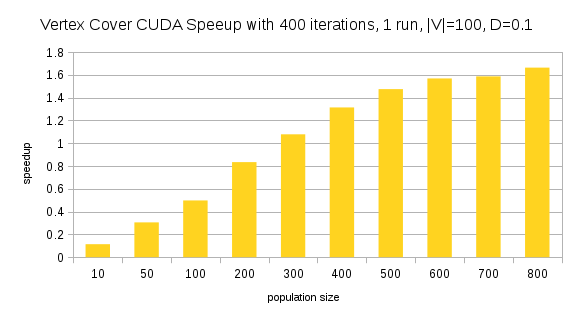
\includegraphics[width=.9\textwidth]{vc_change_pop.png}
  			\caption{Speedup for Vertex Cover, varying population size}
		\end{figure}
	\end{frame}
	\begin{frame}
		\frametitle{Graphs (2)}
		\begin{figure}[t]
  			\centering
  			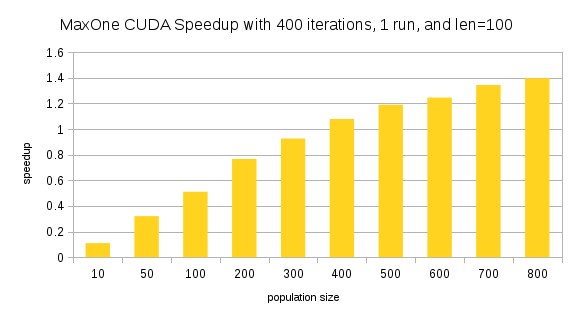
\includegraphics[width=.9\textwidth]{maxone_change_pop.png}
  			\caption{Speedup for MaxOne, varying population size}
		\end{figure}
	\end{frame}
	\begin{frame}
		\frametitle{Graphs (3)}
		\begin{figure}[t]
  			\centering
  			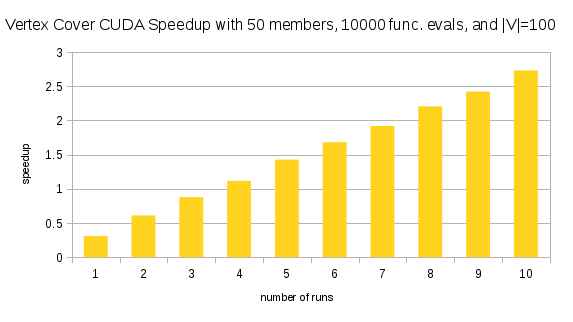
\includegraphics[width=.9\textwidth]{vc_change_runs.png}
  			\caption{Speedup for Vertex Cover with graph density = 0.1, varying the number of runs}
		\end{figure}
	\end{frame}
	\begin{frame}
		\frametitle{Graphs (4)}
		\begin{figure}[t]
  			\centering
  			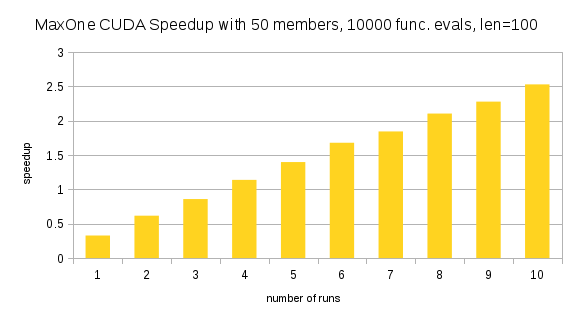
\includegraphics[width=.9\textwidth]{maxone_change_runs.png}
  			\caption{Speedup for MaxOne, varying the number of runs}
		\end{figure}
	\end{frame}
	\begin{frame}
		\frametitle{Graphs (5)}
		\begin{figure}[t]
  			\centering
  			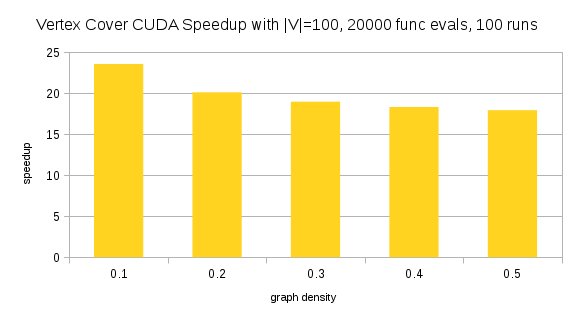
\includegraphics[width=.9\textwidth]{khuri_exper_100.png}
  			\caption{Speedup for Vertex Cover experiment in paper, with $|V|=100$. Unable to do for $|V|=200$ because sequential takes \textbf{very} long to finish}
		\end{figure}
	\end{frame}
\end{document}